%\documentclass{article}
\documentclass[aps,prl,reprint,onecolumn,superscriptaddress,floatfix,longbibliography]{revtex4-2}

\usepackage[utf8]{inputenc}

\title{Quantum particles in fractal external potential}
%\author{astrakharchik }
\date{\today}

\usepackage{natbib}
\usepackage{graphicx}
\usepackage{amsmath}

\begin{document}

\maketitle

\section{Introduction}
The aim of the project is to study the properties of quantum particles in an external field reproducing a fractal structure. A possible realization is an ultracold quantum gas confined to two dimensions with a superimposed external field, which will create the fractal geometry. As a model for the fractal, we will consider Sierpiński carpet. The main properties of interest in the ground state energy and the density profile. Such properties are to be calculated as a function of the recursion number and a possible existence of a simple scaling law has to be verified. 
%\bibliographystyle{plain}
%\bibliography{references}

This interdisciplinary problem is based on application of mathematical concepts to the field of quantum physics and relies on use of numerical methods. This project requires carrying out a scientific investigation and a priori it is not clear which method will work the best. In particular, possible  approaches to address the problem are:
\begin{enumerate}
  \item to solve Schrödinger equation in imaginary time for one particle.
  \item to solve Gross-Pitaevskii equation to solve Schroedinger equation in imaginary time for many bosons.
  \item do exact diagonalization of a discretized Hamiltonian for one particle and few fermions.
  \item random walks solution for the diffusion equation (i.e. Schroedinger equation in imaginary time) for one particle.
\end{enumerate}

\section{Literature overview}

\cite{Sierpinski1916}

The transport through fractal surface attracts a lot of theoretical and experimental attention. 
The flow of a classical fluid though Sierpinski carpet seen as a porous medias has been considered in Ref.~\cite{Li2011}. 
It was found that tortuosity $\tau$ of flow paths (ration between the full length of the full path to the displacement) increases with iteration number $n$ of the fractal as $\tau_n = (19/18)^n$. 
At the same time the porosity (accessible fraction of the volume) decreases as $\phi = (8/9)^n$.
Quantum transport recently has been studied in Sierpinski carpet~\cite{vanVeen2016} and experimentally measured in Sierpinski triangle fractal~\cite{Kempkes2018}.
Edge modes have been studied in Ref.~\cite{Fremling2020,fischer2021robustness}.

Typically tight-binding approximation is 
used\cite{vanVeen2016,Kempkes2018,xu2020shining,Fremling2020}

The scaling theory of localization was first introduced in \cite{Abrahams1979}

\section{Complexity of the problem}

It has been noted that the complexity grows exponentially with the iteration $n$ of the fractal. 
In Ref.~\cite{Li2011} it was reported that calculations for $n=5$ were taking several hours and for $n=6$ more than week of computational time.
Graphic Processor Units (GPUs) have been used in order to make a parallel calculation of the diffusion in Siepinski carpet more efficient in Ref.~\cite{Hoffmann2010}.

It can be also noted that some authors have applied random walks\cite{Janaswamy2007,Kolluru2008} and neural networks for solving a related problem of Laplace equation

\break  
\section{Solving Schrödinger equation for a particle in a box with an external potential with a Sierpinski shape}

We are applying an external potential with a Sierpinski fractal shape to a particle and solving the Schrödinger equation numerically to obtain the wave function and its ground energy.

\subsection{Zero boundary conditions}

One possibility is to impose zero boundary conditions (z.b.c.). 
To do so, we define a box with a side length of $L=1$ centered at the origin and apply Dirichlet boundary conditions that define a value of the solution, $f(x,y)=0$, on the border area. 
Physically such conditions correspond to a hard wall of an infinite size, so that particle cannot escape the box.

A single quantum particle in a box with zero boundary conditions has a finite energy equal to 
\begin{equation}
E_{box,zbc} = \frac{\pi^2\hbar^2}{mL^2}
\label{Eq:E:zbc}
\end{equation}

\subsection{Periodic boundary conditions}
Another possibility is to use periodic boundary conditions (p.b.c.).
In this case we use a box with a side length of $L=1$ centered at the origin and apply von Neumann boundary condition 
\begin{equation}
\frac{\partial }{\partial x} f(|x|=L/2,y)= 0
\label{Eq:pbc:x}
\end{equation}
and
\begin{equation}
\frac{\partial }{\partial y} f(x,|y|=L/2) = 0\;.
\label{Eq:pbc:y}
\end{equation}
Conditions~(\ref{Eq:pbc:x}-\ref{Eq:pbc:y}) are equivalent to periodic boundary conditions.

Physically, periodic boundary conditions provide a faster convergence to the thermodynamic limit when the box size is increased. 
Indeed, for any box size $L$, the ground-state energy of a single particle is equal to its thermodynamic value, 
\begin{equation}
E_{box,pbc} = 0\;,
\label{Eq:E:pbc}
\end{equation}
contrarily to $1/L^2$ dependence observed in the case of zero boundary conditions~(\ref{Eq:E:zbc}). 
Excitation spectrum in a box with periodic boundary conditions is
$E_{n_x, n_y} = \frac{2\pi^2\hbar^2(n_x^2+n_y^2)}{mL^2}$ where $n_x = 0;\pm 1; \pm 2;\cdots$ and 
$n_y = 0;\pm 1; \pm 2;\cdots$ are quantum numbers of excitations along two directions.

\subsection{Solve Schrödinger equation}
Now, we need to solve the time-independent Schrödinger equation.
\begin{equation}
\hat {H} |\Psi \rangle = E |\Psi \rangle
\end{equation}
We can see how $E$ is the eigenvalue of $\Psi$ when $\hat{H}$ acts on $\Psi$. That means that if we can define the Hamiltonian in a matrix way, we can solve it by finding the eigenvalues and eigenvectors of the matrix.\\
As we want to solve it for a particle on the plane, the Hamiltonian operator has 2 dimensions.\\
\begin{equation}
\hat {H} = \hat {T} + \hat {V} = -\frac{\hbar^{2}}{2m} \nabla^{2} + \mathbf{V}
\end{equation}
We want to study the effect of the Sierpinski shaped external potential, so on these solution we are going to leave out the mass and the $\hbar^{2}$ by the moment.\\
The Laplace operator acting on a function $f$ is equal to the sum of the second derivatives of $f$.
We are going to solve these equation in a discrete space, and the multidimensional discrete Laplacian operator is a Kronecker sum of one dimension discrete Laplacians. Using the finite-difference method we can define a second derivative of a function $f$ like:
\begin{equation}
\frac{\partial^{2}f}{\partial x^2} \approx \frac{f_{i-1} - 2f_{i} + f_{i+1}}{\Delta x^{2}}
\end{equation}
The Kronecker sum of two discrete Laplacians is defined as:
\begin{equation}
\mathbf{L}=\mathbf{D_{xx}} \oplus \mathbf{D_{yy}}=\mathbf{D_{xx}} \otimes \mathbf{I} + \mathbf{I} \otimes \mathbf{D_{yy}}
\end{equation}
where $\mathbf{D_{xx}}$ and $\mathbf{D_{yy}}$ are one dimensional discrete Laplacians in the x and y-directions correspondingly, and $\mathbf{I}$ is the identity matrix of appropriate size.\\
In the case of Zero boundary conditions, we define the matrix $\mathbf{D_{xx}}$ like:
\begin{equation}
\mathbf{D_{xx}} = \frac{1}{\Delta x^{2}}
\begin{pmatrix} 
-2 & 1 & & & \\
1 & -2 & 1 & & \\
& \ddots & \ddots & \ddots &  \\
& & 1 & -2 & 1 \\
& & & 1 & -2
\end{pmatrix}
\end{equation}
As I explained earlier, our border conditions are that the wavefunction outside the box has a value of 0, what means that $\psi_{i,0} = \psi_{i,n + 1} = \psi_{0,i} =  \psi_{n + 1,i} = 0$ for all $0 \leq i \leq n$.\\
Now, defining $\mathbf{D_{yy}}$ the same way as $\mathbf{D_{xx}}$ but with ${\Delta y^{2}}$, we can compute the discrete Laplacian as the matrix $\mathbf{L}$ and define the Hamiltonian with a matrix form.
\begin{equation}
\mathbf{L} = \mathbf{D_{xx}} \oplus \mathbf{D_{yy}}
\end{equation}
\begin{equation}
    \mathbf {H} = \mathbf{L} + \mathbf{V}
\end{equation} 
\begin{equation}
\mathbf{L}\psi + \mathbf {V}\psi = \mathbf {E}\psi
\end{equation} 
Now, we end up solving the equation (12) by finding the eigenvalues and eigenvectors of the $\mathbf{H}$ matrix.\\
Periodic boundary conditions can be as well imposed in the discrete form. In this case, matrix $\mathbf{D_{xx}}$ has two additional elements on positions $(N,1)$ and $(1,N)$:
\begin{equation}
\mathbf{D_{xx}} = \frac{1}{\Delta x^{2}}
\begin{pmatrix} 
-2 & 1 & & & 1 \\
1 & -2 & 1 & & \\
& \ddots & \ddots & \ddots &  \\
& & 1 & -2 & 1 \\
1 & & & 1 & -2
\end{pmatrix}
\end{equation}

\subsection{Degenerate eigenvectors}

In the special case when the Hamiltonian has degenerate eigenstates, the inverse participation ratio criterion has to be reconsidered as depending on which specific combination is considered, the result can be different.

In order to test if this is the case, we consider the generic eigenvalue problem,
\begin{equation}
\hat H|\psi_i\rangle = E_i|\psi_i\rangle,
\end{equation}
where index $i$ counts different eigenvalues. The action of the Hamiltonian $\hat H$ to a state $|\psi_i\rangle$ can be intepreted in vector form as some rotation and stretching of the vector, 
\begin{equation}
|\psi'\rangle = H|\psi\rangle. 
\end{equation}
If the vector $|\psi\rangle$ is an eigenvector, its direction is not changed so that $|\psi'\rangle$ and $|\psi\rangle$ are parallel,
\begin{equation}
\frac{\langle \psi'|\psi\rangle^2}{\langle \psi'|\psi'\rangle\langle \psi|\psi\rangle} = 1
\end{equation}
and the change in the normalization is governed by the eigenvalue $E$,
\begin{equation}
\frac{\langle \psi'|\psi'\rangle}{\langle \psi|\psi\rangle} = E^2
\end{equation}

In the case when several eigenvalues are degenerate, for example 
$E_0 = E_1 = E_2 = E_3$, any linear combination of corresponding eigenvectors such as
$|\psi\rangle = C_0|\psi_0\rangle+C_1|\psi_1\rangle+C_2|\psi_2\rangle+C_3|\psi_3\rangle$ where $C_0,\cdots,C_3$ are some coefficients, is again an eigenvector, i.e. $\hat H|\psi\rangle= E_0|\psi\rangle$.

If some vector is ``almost'' an eigenvector, 
$|\psi'\rangle \approx H|\psi\rangle$ its direction will almost remain the same, i.e.  
\begin{equation}
\frac{\langle \psi'|\psi\rangle^2}{\langle \psi'|\psi'\rangle\langle \psi|\psi\rangle} \approx 1
\end{equation}
and the change in the normalization will be almost the eigenvale $E$,
\begin{equation}
\frac{\langle \psi'|\psi'\rangle}{\langle \psi|\psi\rangle}\approx E^2
\end{equation}

\section{Diffusion coefficient.}

Brownian motion of a particle, in which its position is randomly changed, in a free space leads to a linear time dependence of the mean square displacement, 
\begin{equation}
\langle r^2(t)\rangle \propto t,
\label{Eq:Einstein}
\end{equation}
and can be seen as a direct consequence of the central limit theorem.
The linear relation~(\ref{Eq:Einstein}) is known as the Einstein's diffusion relation. 
It was found in Ref.~\cite{Hoffmann2010} that a diffusion in a discrete Sierpinski carpet (particle hops between squares of the minimal size) does not follow the usual Einstein's relation, $\langle r^2(t)\rangle\propto t$, but is rather follows the anomalous diffusion law\cite{MetzlerKlafter2000},
\begin{equation}
\langle r^2(t)\rangle \propto t^\gamma,
\end{equation}
where $0<\gamma<1$ is the diffusion exponent. 

Another important quantity is the probability density $P(r,t)$ representing the probability that a particle is found at distance $r$ from the original position after it has travelled time $t$. 
Diffusion on Sierpinski gasket is given by the scaling form, known as a stretched Gaussian\cite{EduardoRoman1995}
\begin{equation}
P(r,t)\propto A(\alpha,\beta) \xi^\beta \exp(-c\xi^u),
\end{equation}
where $\xi = r/t^{\alpha/2}$, $u=1/(1-\alpha/2)$ and $\beta$ depends on the system type. For subdiffusion, $0<\alpha<1$, and $0<u<2$.[224]
Renormalization group theory was used for this system resulting in a relation between the fractal dimensions and critical exponents\cite{Guyer1984}.

For Sierpinski carpet $P(r,t)\propto t^{-1/2} r^{D-n}\exp(-cr^{2D}/t)$ where $D=\ln 8/\ln 3$
$d_s = 1.805$.

There are two types of random process. A random walk in a fractal can be described as a random walk of an ant in a labyrinth. There are two types of ants: blind and miopic\cite{FRANZ2000}. A blind ant tries to move in all directions and stays blocked in a certain step if the move is not possible. A miopic and instead sees allowed directions and always moves at each step.
%% new algorithm?
% DOI:10.1088/0305-4470/33/5/001
% critical exponenrts?
% https://iopscience.iop.org/article/10.1088/0305-4470/32/37/302
% On the propagator of Sierpinski gaskets J Klafter1, G Zumofen1 and A Blumen1

%

\section{Results}

\begin{figure}[h!]
    \centering
    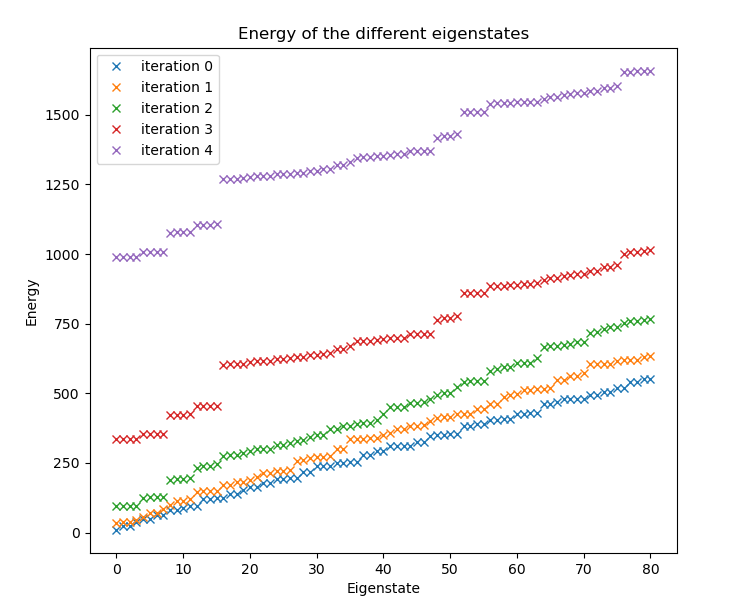
\includegraphics[scale=0.5]{./images/energy_eigenstates.png}
    \caption{The energy of lowest eigenstates for different iterations of the fractal, with N = 81}
    \label{figure:IPR}
\end{figure}

\begin{figure}[h!]
    \centering
    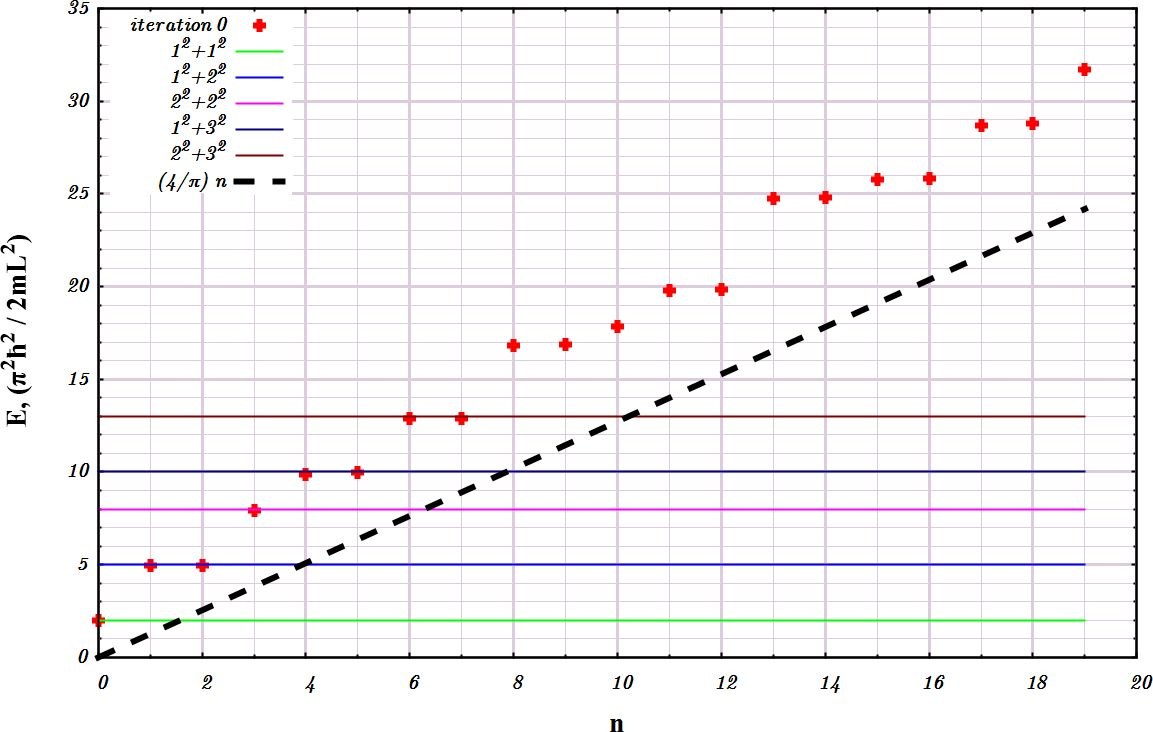
\includegraphics[scale=0.5]{./images/FigEiter0.jpg}
    \caption{The energy of lowest eigenstates for zeroth iteration as compared to Eq.~(\ref{Eq:E:zbc})}
    \label{figure:IPR}
\end{figure}

For the zeroth iteration (i.e. no external field) the problem can be solved exactly, resulting in energy
\begin{equation}
E = \frac{\pi^2\hbar^2}{2mL^2}(n_x^2+n_y^2),
\end{equation}
and eigenstates
\begin{equation}
\phi(x,y) = \sin\left(\frac{\pi n_x x}{L}\right)\sin\left(\frac{\pi n_y y}{L}\right)
\end{equation}
with $\{n_x,n_y\}=1,2,\cdots$. 
Quantum numbers $n_x$ correspond to the average square momentum
\begin{equation}
\langle p_x^2\rangle 
= 
-\langle \hbar^2 \frac{\partial^2}{\partial x^2}\rangle 
= \frac{\pi^2 n^2}{L^2}
\end{equation}
Energy as a function of the number of the eigenstate $n$ can be approximately calculated by assuming a uniform distribution of the eigennumbers. 
The number of the eigenstate roughly corresponds to one fourth of the area $\pi n_x^2$ of the circle in $(n_x, n_y)$ plane, i.e $n\approx \pi n_x^2$
\begin{equation}
E = \frac{\pi^2\hbar^2}{2mL^2} \frac{4n}{\pi}
\label{Eq:E:zbc}
\end{equation}

\begin{figure}[h!]
    \centering
    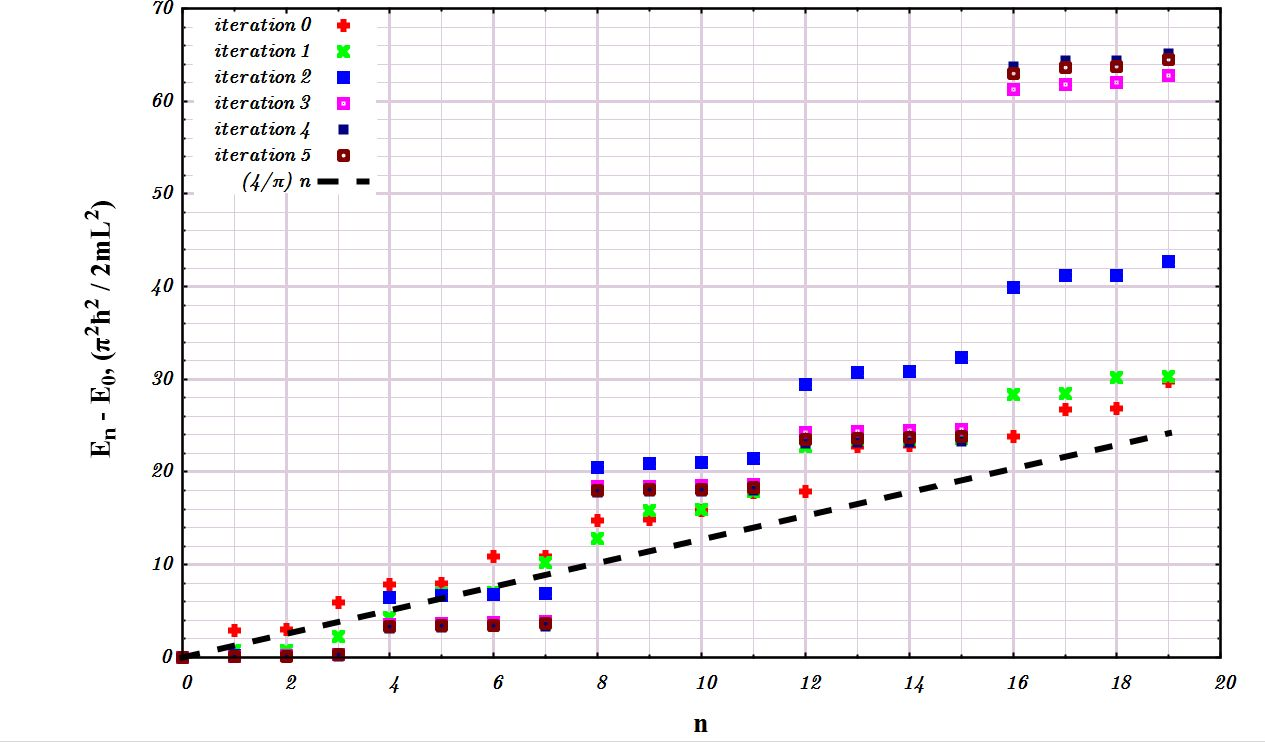
\includegraphics[scale=0.5]{./images/FigEiter.jpg}
    \caption{The energy of lowest eigenstates $E_n-E_0$ for different iterations
    }
    \label{figure:IPR}
\end{figure}







\section{Bibliography}
\bibliography{bibliography}

%\break
%\begin{thebibliography}{9}
%\bibitem{} https://en.wikipedia.org/wiki/ Sierpinski Carpet
%\bibitem{} https://en.wikipedia.org/wiki/Schrodingerequation
%\bibitem{} https://en.wikipedia.org/wiki/Gross-Pitaevskii equation
%\bibitem{} Simulating the 1D GPE http://link.springer.com/content/pdf/bbm\%3A978-3-319-42476-7\%2F1.pdf
%\bibitem{} Solving Hydrogen atom numerically with 14 lines of Matlab code https://timqian.com/2015/03/04/H-atom-numerical

%\bibitem{}https://sci-hub.se/10.1007/978-3-319-05053-9

%[Kolluru2008] SH Kolluru, Preliminary Investigations of a Stochastic Method to solve Electrostatic and Electrodynamic Problems. Masters Thesis, UNIVERSITY OF MASSACHUSETTS AMHERST, August 2008, http: //scholarworks.umass.edu/cgi/viewcontent.cgi?article=1261&context=theses
%\end{thebibliography}

\end{document}